
\section{Prueba de Concepto}
Para la realización de este proyecto se ha decidido crear un entorno virtual dentro de la infraestructura real donde está localizado el servicio, para poder desplegar el software Cloud Foundation y probarlo sin afectar a la configuración ni al funcionamiento general del servicio. La parte física de este entorno está formada por cuatro máquinas virtuales, que equivalen a cuatro nodos físicos con el hipervisor ESXi instalado en cada uno. También cuenta con una máquina virtual con vCenter Server para permitir el acceso al entorno, y otra máquina virtual con Windows Server 2016 donde se habilitan servicios de red como DNS,NTP o DHCP.
*****ESTRUCTURA DEL ENTORNO.
\subsection{Especificaciones del entorno}
Estas son las características de hardware y software del nuevo entorno de pruebas.
\begin{itemize}
    \item \textbf{Cuatro nodos ESXi}, cada uno con la siguiente configuración:
    \begin{itemize}
        \item Hipervisor: VMware ESXi, version 6.7.0, build 10302608
        \item Procesador: Intel(R) Xeon(R) CPU E5-2650 v4 @ 2.20GHz
        \item Memoria: 24GB
        \item Discos de almacenamiento: un disco duro arranque con 8GB de capacidad, un disco duro de 100GB y tres discos duros de 200GB.
    \end{itemize}
            \begin{figure}[h!]
            \centering
            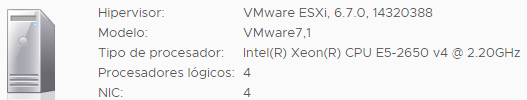
\includegraphics[width=0.85\textwidth]{imaxes/probaConcepto/caracteristicas_NODO.png}
            \caption{Características comunos a cada host.} 
            \label{fig:caracteristicasNODO}
        \end{figure}
        \FloatBarrier
    \item \textbf{Almacenamiento}: El almacenamiento está basado en el prodcuto VMware vSAN siguiendo el modelo All-Flash. Este servicio unifica los discos duros de cada host en un único almacén de datos dividido en cuatro grupos de discos donde el disco de 100 GB representa el disco de memoria caché y los tres discos de 200 GB representan los discos de capacidad. La capacidad total útil del clúster es de 2,34 TB.
    \item \textbf{Software}: Para crear la capa de virtualización, este entorno tiene instalado vSphere que contiene los componentes ya descritos [Sec.\ref{subsec:softwareinstalado}], y vSAN para la gestión del almacenamiento [Sec. \ref{subsubsect:cfcomponents}].
\end{itemize}

\subsection{Configuración Inicial}
En este apartado se expone cual es la configuración de los nodos físicos sobre red y servicios habilitados antes de realizar el despliegue de Cloud Foundation. Nodos existentes:
%%%%%%Centrar esta lista.%%%%%%%%%%%
    \begin{itemize}
        \item \textbf{Nodo 1}: sa-esxi-01.vclass.local
        \item \textbf{Nodo 2}: sa-esxi-02.vclass.local
        \item \textbf{Nodo 3}: sa-esxi-03.vclass.local
        \item \textbf{Nodo 4}: sa-esxi-04.vclass.local
    \end{itemize}
%%%%%%%%%%%%%%%%%%%%%%%%%%%%%%%%%%%

\subsubsection{Red}
\label{sec:redPrueba}
Los cuatro nodos del entorno están conectados entre si a través de tres redes, cada una con un propósito diferente. Para la distribución de los datos de cada red, se utiliza un switch virtual llamado vSwitch que da conectividad entre las máquinas virtuales y hosts del entorno (un vSwitch por red). Cada nodo tiene cuatro puertos físicos, que en este caso son virtuales ya que los nodos no son reales, los cuales se asignan a los diferentes vSwitches que se van creando para configurar la red, permitiendo asignar más de un puerto a un vSwitch para crear redundancia. Así, cada vSwitch redirigirá el tráfico por su puerto asignado. Dentro de la nomenclatura de VmWare, estos puertos se llaman \setword{\textbf{vmnicX}}{Word:vmnic} donde X es su numeración.\\
Configuración de los switches en cada nodo, esta configuración se repite en cada nodo:
\begin{itemize}
    \item \underline{vSwitch0}:
    \label{itm:managementNet}
        Red \emph{SDDC-DPortGroup-Mgmt} con IP 172.20.10.0/24.
        El nodo 1 tiene la IP 172.20.10.51, el nodo 2 la IP 172.20.10.52, el nodo 3 la IP 172.20.10.53, y el nodo 4 la IP 172.20.10.54.
        Esta red es utilizada por servicios de gestión, como el acceso SSH a los nodos, la sincronización de tiempo por NTP, acceso al servidor DNS, o el acceso a la interfaz de configuración del entorno con vSphere WebClient. Se usa a través de puertos \emph{vmkernel}.

        \begin{figure}[h!]
            \centering
            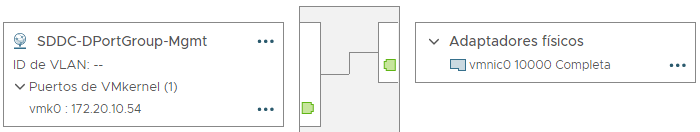
\includegraphics[width=0.85\textwidth]{imaxes/probaConcepto/vswitch0.png}
            \caption{\emph{vSwitch0} del nodo \emph{sa-esxi-01.vclass.local}} 
            \label{fig:componentesVSphere}
        \end{figure}
        \FloatBarrier
    \item \underline{vSwitch1}:
    \label{itm:vsanNet}
        Red \emph{SDDC-DPortGroup-VSAN} con IP 172.20.12.0/24.
        El nodo 1 tiene la IP 172.20.12.51, el nodo 2 la IP 172.20.12.52, el nodo 3 la IP 172.20.12.53, y el nodo 4 la IP 172.20.12.54.
        Esta red sirve para comunicar los nodos con el datastore de vSAN. Se usa a través de puertos \emph{vmkernel}.
        \begin{figure}[h!]
            \centering
            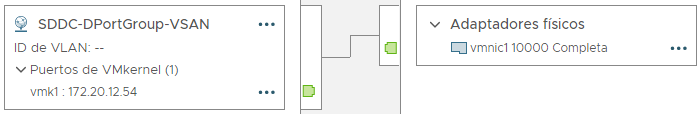
\includegraphics[width=0.85\textwidth]{imaxes/probaConcepto/vswitch1.png}
            \caption{\emph{vSwitch1} del nodo \emph{sa-esxi-04.vclass.local}} 
            \label{fig:componentesVSphere}
        \end{figure}
        \FloatBarrier
    \item \underline{vSwitch2}:
    \label{itm:machinesNet}
        Red \emph{VM Network}. No tiene ninguna IP asignada. Esta red da conectividad a las máquinas virtuales de cada nodo. Se usa a través de puertos \emph{vmportgorups}.
        \begin{figure}[h!]
            \centering
            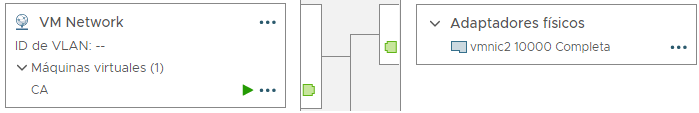
\includegraphics[width=0.85\textwidth]{imaxes/probaConcepto/vswitch2.png}
            \caption{\emph{vSwitch2} del nodo \emph{sa-esxi-04.vclass.local}} 
            \label{fig:componentesVSphere}
        \end{figure}
        \FloatBarrier
\end{itemize}

******ESQUEMA DE LOS PUERTOS**************

 Según el tipo de red que se esté añadiendo en cada vSwitch, se creará en este un tipo distinto de puerto que se conectará con el puerto físico mencionado anteriormente. Estos puertos pueden ser \setword{\emph{vmwkernel}}{Word:vmkernel} (vmkX) para el tráfico de los servicios que usan los nodos ESXi, y \textit{vmportgroup} para tráfico general de las máquinas virtuales.
 Para que un nodo tenga conectividad con otro nodo, estos deben tener configurada la misma red en sus vSwitches. 
 Inicialmente, todas las redes tienen deshabilitado el etiquetado de VLAN.\\
 Estos vSwitches descritos forman la red lógica del entorno pero por donde realmente viaja todo el tráfico es sobre la red física de la infraestructura, que está formada por un switch cuyo MTU es igual a 1500.
 
 
 \subsubsection{Servicios internos}
 
 Inicialmente, en cada host los siguientes servicios están configurados y en ejecución:
 \begin{itemize}
     \item \textbf{Direct Console UI}: permite interactuar con el host de forma local mediante una interfaz basada en texto.
     \item \textbf{ESXi Shell}: permite interactuar con los hosts de forma completa, ya sea en local o en remoto, mediante comandos. Se puede acceder a través de SSH.
     \item \textbf{SSH}: servicio que habilita el acceso a ESXi Shell de forma remota.
     \item \textbf{Load-Based Teaming}: establece una política para balancear el tráfico que pasa por cada puerto \emph{vmnic}.
     \item \textbf{NTP}: servicio que obtiene la hora actual de un servidor NTP, así todos los nodos mantienen su hora sincronizada. La sincronización se realiza con un servidor NTP con la IP 172.20.10.10.
     \item \textbf{Syslog Server}: recoge mensajes de VMkernel y otros componentes.
     \item \textbf{VMware vCenter Agent}: permite al vCenter tener acceso a cada nodo.
     \item \textbf{DNS}: servicio que está situado en un servidor con la IP 172.20.10.10. Contiene todas las redes exitentes y los nombres de cada host para que todos los componentes sean accesibles a través de la red.
 \end{itemize}
 En el entorno existe un dominio de \emph{Single Sing-On}[\ref{itm:singlesingonEX}] habilitado con el nombre \emph{vsphere.local}.\\
 
 \subsubsection{Servicios externos}
 El servidor donde se encuentran los servicios DNS, DHCP y NTP, tiene tres adaptadores de red a donde llegan cada una de las redes descritas anteriormente.\\
 El \underline{servicio DNS} cuenta con los siguientes nombres registrados:
         \begin{figure}[h!]
            \centering
            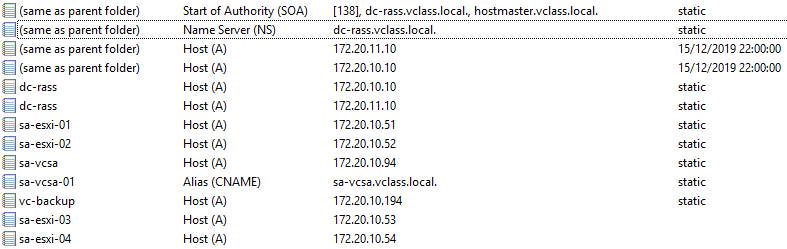
\includegraphics[width=0.95\textwidth]{imaxes/probaConcepto/nombresDNSINIcioFW.png}
            \caption{Contenido inicial \textit{forward} del DNS.} 
            \label{fig:contenidoinicialForwardDNS}
        \end{figure}
        
        \begin{figure}[h!]
            \centering
            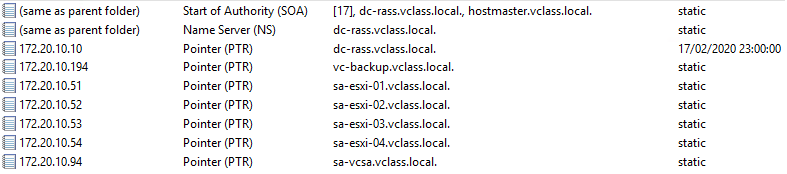
\includegraphics[width=0.95\textwidth]{imaxes/probaConcepto/dnsINICIOReverse.png}
            \caption{Contenido inicial \textit{reverse} del DNS.} 
            \label{fig:contenidoinicialReverseDNS}
        \end{figure}
        \FloatBarrier
El \underline{servicio DHCP} cuenta con la siguiente configuración:
        \begin{figure}[h!]
            \centering
            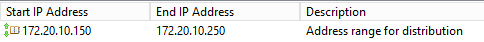
\includegraphics[width=0.85\textwidth]{imaxes/probaConcepto/scope1722010Inicio.png}
            \caption{Rango de IPs inicial para la red de 172.20.10.0/24 (Descrip. \ref{itm:managementNet}).} 
            \label{fig:dhcpInicioManage}
        \end{figure}
        \begin{figure}[h!]
            \centering
            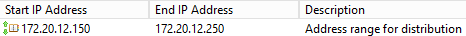
\includegraphics[width=0.85\textwidth]{imaxes/probaConcepto/scope1722012Inicio.png}
            \caption{Rango de IPs inicial para la red de 172.20.12.0/24 (Descrip. \ref{itm:vsanNet}).} 
            \label{fig:dhcpInicioSAN}
        \end{figure}
        \begin{figure}[h!]
            \centering
            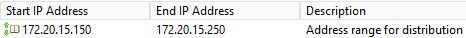
\includegraphics[width=0.85\textwidth]{imaxes/probaConcepto/scope1722015Inicio.png}
            \caption{Rango de IPs inicial para la red de 172.20.15.0/24 (Descrip. \ref{itm:machinesNet}).} 
            \label{fig:dhcpInicioMachines}
        \end{figure}
    \iffalse
        \begin{figure}[h!]
            \centering
            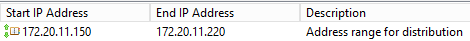
\includegraphics[width=0.85\textwidth]{imaxes/probaConcepto/scope1722011Inicio.png}
            \caption{Rango de IPs inicial para la red de 172.20.11.0/24 (Descrip. \ref{itm:machinesNet}).} 
            \label{fig:dhcpInicioMachines}
        \end{figure}
    \fi
    Para dar acceso a estos tres servicios desde cualquier componente del entorno el servidor donde se encuentran alojados debe tener al menos un adaptador de red (NIC) por cada red existente. Además, este servidor es la puerta de enlace de todos los componentes por lo que también se debe modificar su tabla de enrutamiento y para que todos los componentes del entorno se puedan comunicar entre si.\\
    *******METER FOTO DE LOS ADAPTADORES DE RED**********\\
    *******METER FOTO DE LA TABLA DE ENRUTAMIENTO.*********
    
\FloatBarrier
    % Las interfaces de cada router lógico son de los siguientes tipos:
    
    % \begin{itemize}
    %   \item \textit{External Interface}: se refiere a las interfaces que conectan con el dispositivo de la red física, normalmente un router.
    %   \item \textit{Internal Transit Link}: está interfaz conecta a todos los DR de \textit{Tier-0} distribuídos en cada TN con los SR formando una única red.
    %   \item \textit{RouterLink Interface}: interfaz que conecta un router lógico de \textit{Tier-1} con uno de \textit{Tier-0} a través de una subred generada por defecto (100.64.0.0/16).
    % \end{itemize}
    
    % Los routers lógicos creados para el \textit{management domain} en el entorno tienen la siguiente configuración:
    
    % \begin{itemize}
    %   \item \textbf{mgmt-domain-tier0-gateway}: su función consiste en proporcionar acceso a la red física.
    %     \begin{itemize}
    %       \item \textit{External Interfaces}\footnote{Estas direcciones corresponden a las interfaces de los TN NSX-T Edge que conectan con las interfaces Uplink sobre dos \textit{segments} de tipo VLAN.}: Dos que se conectan al \textit{segment} \textit{VCF-edge\_mgmt-edge-cluster-segment-11} (172.27.11.2 y 172.27.11.3) y dos que se conectan al \textit{segment} \textit{VCF-edge\_mgmt-edge-cluster-segment-12} (172.27.12.2 y 172.27.12.3).
    %       \item \textit{Internal Transit Link}: Usa la subred 169.254.0.0/24.
    %       \item \textit{RouterLink Interface}: Tiene la dirección 100.64.192.0/31.
    %       \item Configuración: se 
    %       \item Configuración HA: determina el modo en el que se va a ejecutar el router de \textit{Tier-0}. En este caso se selecciona el modo \textit{active-active} el cual implica que las instancias de SR (una en cada nodo NSX-T Edge) funcionan ambas de forma activa, el tráfico que reciba cada una será encaminado por una subred diferente. Es por esto que el router lógico de \textit{Tier-0} no puede ofrecer servicios centralizados.
    %     \end{itemize}
    
    %   \item \textbf{mgmt-domain-tier1-gateway}: router de \textit{Tier-1} dedicado a gestionar el enrutamiento de las VMs de aplcaciones no dedicadas a la administración del SDDC. 
    %   \begin{itemize}
    %     \item \textit{Internal Transit Link}: Usa la subred 164.254.0.0/24.
    %     \item \textit{RouterLink Interface}: Tiene la dirección 100.64.192.1/31.
    %     \item \textit{Segment Interfaces}: conectado al \textit{segment} \textit{mgmt-Region01A-VXLAN} con la dirección IP 10.50.0.1, y al \textit{segment} \textit{mgmt-xRegion01-VXLAN} con la dirección IP 10.60.0.1.
    %     \item Configuración HA: determina el modo en el que se va a ejecutar el router de \textit{Tier-1}. En este caso se selecciona el modo \textit{active-stanby} el cual solo utiliza una de las dos instancias del SR de \textit{Tier-1} (cada una en un nodo de NSX-T Edge) por lo tanto el tráfico que reciba solo será encaminado por un único punto. Esto permite activar servicios centralizados, por lo tanto será \textit{mgmt-domain-tier1-gateway} y no \textit{mgmt-domain-tier0-gateway} el encargado de proporcionarlos.
    %   \end{itemize}
    % \end{itemize}
    
    % Así como el componente DR de los routers de \textit{Tier-0} y de \textit{Tier-1} están distribuídos por todos los TNs (incluídas las instancias de NSX-T Edge), el componente SR solo se encuentra en las VMs de NSX-T Edge por lo tanto son estas VMs las que proporcionan los servicios centralizados de SR y acceso a la red externa del entorno. Además, para que los componentes lógicos tengan acceso a los \textit{segments} descritos, las instancias de NSX-T Edge están conectadas a dos TZs:
    % \begin{itemize}
      
    %   \item \textit{mgmt-domain-m01-overlay-tz}: esta TZ proporciona a las VMs del entorno a los servicios de los routers de \textit{Tier-0} y de \textit{Tier-1} y también permite que esos routers lógicos tengan acceso a los \textit{segments} donde se encuentran esas VMs. Se utiliza el tipo Overlay para que se puedan comunicar TNs que se encuentran en distintas redes físicas sin que la configuración de la red física sea compleja.
      
    %   \item \textit{sfo01-m01-dge-uplink-tz}: esta TZ se utiliza para conectarse a la red física a través de un router físico. Se utiliza el tipo VLAN para encapsular el tráfico saliente hacia al router físico y porque las VLANs usadas en los \textit{segments} dentro de esta TZ se configuran también en la infraestructura física, por lo tanto no hace falta crear una capa física virtual con Overlay.
    % \end{itemize}
    
    % Para gestionar las conexiones de cada TN, tanto para los nodos NSX-T Edge como para los hosts ESXi, VMware NSX-T introduce el componente llamado \textbf{NSX-T Virtual Distributed Switch} (N-VDS). Cada TN del entorno posee un N-VDS, este elemento conecta sus interfaces a los \textit{segments} que se configuran en cada TN y establece un mapeo con las interfaces \textit{uplink} que se utilizan para dirigir el tráfico de cada TZ hacia el exterior del TN. En el caso de las instancias de NSX-T Edge, los dos \textit{uplinks} están mapeados con las NICs físicas de cada host ESXi a través de los dos \textit{distributed port groups} de vSphere vDS (\textit{sddc-edge-uplink01} y \textit{sddc-edge-uplink02}) a los que están ancladas ambas VMs, es decir, un \textit{uplink} está mapeado con una NIC física del host ESXi. 
    % En las TZ de tipo VLAN, se utilizan plantillas \textit{Uplink Policy} para indicar como debe el N-VDS tratar el tráfico de la \textit{transport zone} a la que se asigna. En cada \textit{Uplink Policy} se especifican varias \textit{Teaming Policy}, el identificador VLAN que debe usar el N-VDS cuando tiene que enviar el tráfico fuera del TN y el MTU de los \textit{uplinks}. Una \textit{Teaming Policy} indica como el N-VDS utiliza los \textit{uplinks} para conseguir conexiones redundantes y balanceo de la carga, en una \textit{Uplink Policy} se especifica una \textit{Teaming Policy} por defecto y otras adicionales.
    % Para la TZ de tipo VLAN \textit{sfo01-m01-dge-uplink-tz} se especifica la siguiente \textit{Uplink Policy}:
    % \begin{itemize}
    %   \item Nombre: \textit{uplink-profile-13}
    %   \item Transport VLAN: 13
    %   \item MTU: 8940
    %   \item Teaming Policy: se especifican tres, una por defecto y dos adicionales:
    %     \begin{itemize}
    %       \item \textit{Default teaming}: \textit{Load Balance Source}, hace un mapeo uno a uno entre cada interfaz virtual de cada VM y uno de los \textit{uplinks} del N-VDS, así todo el tráfico correspondiente a esa interfaz se envía y recibe por el mismo \textit{uplink}.
          
    %       \item \textit{uplink1-named-teaming-policy}: \textit{Failover Order}, se establece un \textit{uplink}, \textit{uplink1} en este caso, como activo que se utiliza para enviar todo el tráfico, y una lista de \textit{uplinks} ordenados que se utilizan en caso de que el primero no esté disponible, vacía para esta \textit{Teaming policy}.
    %       \item \textit{uplink2-named-teaming-policy}: \textit{Failover Order}, donde el \textit{uplink} activo es \textit{uplink2} y la lista de \textit{uplinks} de reserva está vacía.
    %     \end{itemize}
    % \end{itemize}
    % A los \textit{segments} de esta TZ, \textit{VCF-edge-mgmt-cluster-segment-11} y \textit{VCF-edge-mgmt-cluster-segment-12} se les asignan las \textit{Teaming Policy} \textit{uplink1-named-teaming-policy} y \textit{uplink2-named-teaming-policy} respectivamente. Con esta configuración el tráfico de cada \textit{segment} circula por una única NIC física del host ESXi. Esto, junto con la configuración \textit{Failover Order} establecida para los \textit{port groups} \textit{sddc-edge-uplink01} y \textit{sddc-edge-uplink02} en el vSphere vDS,se consigue que el tráfico de salida hacia la red física perteneciente a los componentes de VMware NSX-T y todas las aplicaciones cuya red gestiona VMware NSX-T, sea distribuído por dos redes distintas proporcionando redundancia y disponibilidad del servicio en caso de que ocurra una caída de alguna de las conexiones.
    
    
    
    % Estas conexiones están gestionadas por un N-VDS dentro de cada instancia. Este switch lógico utiliza tres interfaces que se conectan a las diferentes redes lógicas. Para aquellas redes lógicas que requieren salida al medio físico ya sea para comunicarse con otros TN o para acceder a la red externa, el N-VDS utiliza finalmente el switch VDS de VMware vSphere que conecta con las interfaces físicas del host ESXi donde corre la instancia de NSX-T Edge.
    
    % la utilizan tres interfaces para  Estas interfaces son \textit{eth0} que se dedica a la red \textit{Management}, \textit{fp-eth0} y \textit{fp-eth1} que ambas se dedican a la conexión con cada uno de los \textit{segments} Uplink. 
    
    
    % *********************************************
    
    %%%%%%%%
    % Se recomienda que la red física siga una topología de tipo \textit{Leaf-Spine} donde existen swithces que se conectan a los hosts (\textit{leaf switches}), que a su vez se conectan a otra capa de switches (\textit{spine switches}) que finalmente conecta con la red principal del SDDC. Este tipo de topología permite medir mejor su rendimiento y facilita la escalabilidad de la infraestructura. En caso de existir varias AZ, debe existir una red física entre ellas cuya capa 3 funcione con enrutamiento dinámico para automatizar la resolución de problemas en caso de caída de alguna de las conexiones.
    %%%%%%%%%
    
    % \iffalse
    % La información sobre VTEP existentes, la relación entre direcciones MAC de máquinas virtuales y dirección IP de VTEP, y relación entre direcciones MAC de máquinas virtuales y su IP, la poseen las instancias de NSX Controller en tres tablas: 
    %     \begin{itemize}
    %         \item \textit{VTEP Table}, relación entre un VTEP y la VXLAN que tiene acceso: VNI (ID del segmento), IP (dirección IP del VTEP), Segment (dirección IP del segmento), MAC (dirección MAC de la NIC física donde está configurado el VTEP).
    %         \item \textit{MAC Table}, relación entre la dirección MAC de una máquina virtual y el VTEP que le da acceso: VNI (ID del segmento), MAC (dirección MAC de la máquina virtual accesible por la VTEP-IP), VTEP-IP (dirección IP del VTEP que da acceso a la máquina virtual de la MAC indicada).
    %         \item \textit{ARP Table}, relación entre la dirección MAC y la dirección IP de una máquina virtual: VNI (ID del segmento), IP (dirección IP de la máquina virtual), MAC (dirección MAC de la máquina virtual).
    %     \end{itemize}
    % Estas tablas permiten reducir la cantidad de tráfico en la red ya que las máquinas virtuales y dispositivos de enrutamiento ya no requieren enviar tráfico Broadcast para obtenerla.
    % La comunicación directa entre máquinas virtuales situadas en distintos hosts ESXi se realiza con tráfico Unicast entre sus respectivos VTEP, pero una máquina virtual también puede enviar tráfico dirigido a todas las máquinas virtuales que pertenecen a su mismo Logical Switch, es decir, a las máquinas de la misma \textit{trasnport zone}, pero pueden situarse en segmentos de red físicos distintos. Este tipo de tráfico puede ser Multicast, Unknown Unicast y Broadcast (BUM), y en VMware NSX se puede gestionar con tres modos de replicación distintos\footnote{Al configurar un Logical Switch se elige uno de los modos.}, modo Multicast, modo Unicast y modo Híbrido.
    %     \begin{itemize}
    %         \item \textbf{Modo Multicast}: requiere que en la red física se haya configurado una IP multicast para cada VXLAN (es decir, Logical Switch), y el protocolo IGMP Snooping en los switches físicos para crear grupos multicast y que el tráfico sea más eficiente, esto habilita multicast entre los VTEP de la misma subred que el emisor. Para transmitir este tráfico a VTEPs situados en otros segmentos de red, se debe configurar el protocolo PIM para poder enrutarlo con los dispositivos de capa 3 físicos. Esta configuración no permite desacoplar la red lógica de la red física.\\
    %         Se puede establecer un grupo multicast por cada VXLAN, esto implica que un host solo recibirá tráfico si tiene al menos una máquina virtual en el grupo, pero requiere configurar muchos grupos. Otra opción es crear un grupo multicast para todas las VXLAN, se necesitan menos direcciones IP pero se genera más tráfico en la red.
    %     \begin{figure}[h!]
    %     \centering
    %     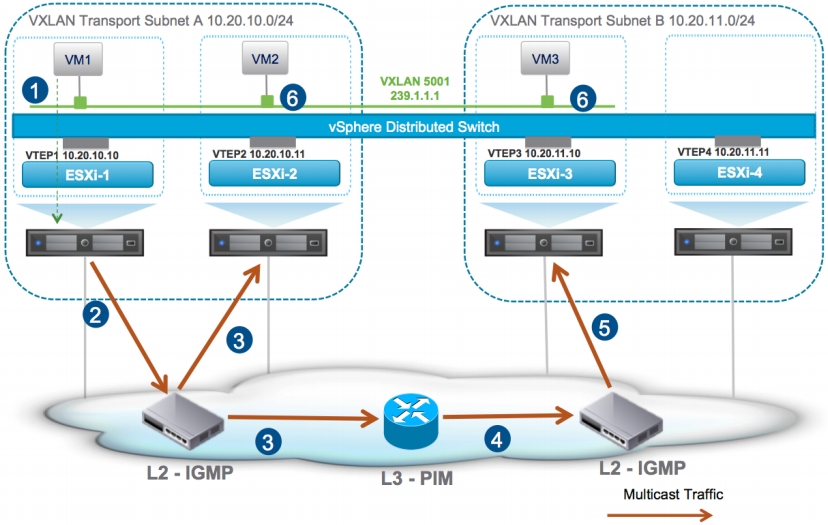
\includegraphics[width=0.5\textwidth]{imaxes/conceptosPrevios/MulticastSeqBUM.png}  \caption{Replicación del tráfico BUM en el modo Multicast}
    %     \label{fig:modoMulticast}
    %     \end{figure}
    %     \FloatBarrier
    %         \item \textbf{Modo Unicast}: no requiere ninguna configuración específica en la capa física y está gestionado por VMware NSX. Se crea un grupo con los VTEP situados en el mismo segmento de red, dentro de cada grupo se selecciona un host ESXi para el rol de \textit{Unicast Tunnel End Point} (UTEP), encargado de recibir el tráfico BUM que procede de otros segmentos de red para reenviarlo por su segmento pero solo a los hosts con al menos una máquina virtual. El host ESXi emisor utiliza la tabla VTEP para comprobar que VTEPs están situados en una VXLAN y así poder dirigir el tráfico BUM correspondiente.\\
    %         Este modo es útil en entornos pequeños donde no hay mucho tráfico y cada segmento de red tiene pocos VTEP.
    %     \begin{figure}[h!]
    %     \centering
    %     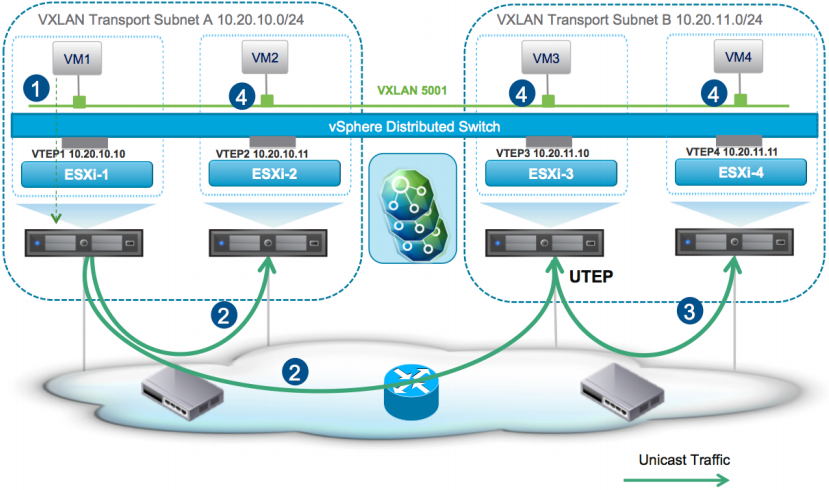
\includegraphics[width=0.5\textwidth]{imaxes/conceptosPrevios/UnicastMode.png}
    %     \caption{Replicación del tráfico BUM en el modo Unicast}
    %     \label{fig:modoUnicast}
    %     \end{figure}
    %     \FloatBarrier
    %         \item \textbf{Modo Híbrido}: combina el modo Unicast y el modo Multicast. El tráfico dirigido a las máquinas virtuales situadas en el mismo segmento de red se transmite usando Multicast, por lo que se requiere tener el protocolo IGMP configurado en los dispositivos físicos de capa 2, se recomienda establecer una dirección Multicast por cada VXLAN. El tráfico se replica a los hosts ESXi que forman parte del grupo. Cuando el tráfico va dirigido a máquinas virtuales situadas en hosts en distinto segmento de red, se transmite utilizando Unicast, como en ese modo, se forma un grupo con los hosts de cada segmento y de cada grupo se elige un host con el rol de \textit{Multicast Tunnel EndPoint} (MTEP). Así, el host que origina el tráfico BUM lo transmite al MTEP correspondiente, el cual se encarga de replicar ese tráfico por su segmento de red. La replicación del tráfico entre segmentos es gestionada por las instancias de NSX Controller.\\
    %         Este modo de replicación permite desplegar NSX en entornos grandes gracias a que el tráfico Multicast y Unicast se pueden escalar facilmente, el primero se reduce a cada segmento de red y la transmisión del segundo en la capa 3 está gestionado por VMware NSX sin necesidad de configurar los dispositivos físicos.
    %     \begin{figure}[h!]
    %         \centering
    %         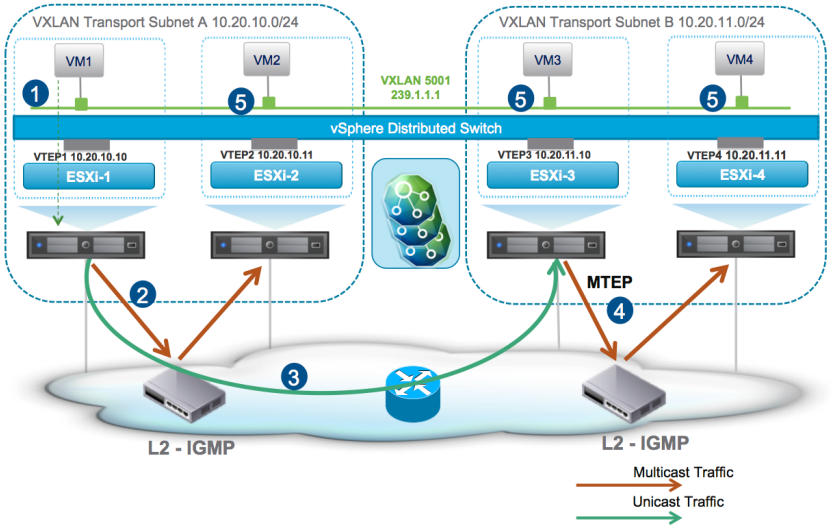
\includegraphics[width=0.5\textwidth]{imaxes/conceptosPrevios/hibrydMode.png}
    %         \caption{Replicación del tráfico BUM en el modo Híbrido}
    %         \label{fig:modoHibrido}
    %     \end{figure}
    %     \FloatBarrier
    %     \end{itemize}
    
    %  El enrutamiento del tráfico está gestionado por dos componentes Distributed Logical Router (DLR) y NSX Edge Services Gateway (ESG). Un mismo DLR se extiende por varios hosts ESXi para enrutar el tráfico entre VXLANs, también mantiene una conexión con las instancias de ESG para transmitir el tráfico que se dirige a redes externas, esa conexión se denomina \textit{transit network} y está getionada por un Logical Switch. Cada DLR tiene su propio Logical Router Control para intercambiar las rutas disponibles con las instancias de ESG, posteriormente, son las instancias de NSX Controller las que transmiten esta información al DLR distribuido en los hosts ESXi. Las interfaces lógicas del DLR conectan con cada Logical Switch, cada interfaz tiene una dirección IP que representa el \textit{gateway} del segmento de red al que esté conectada [Fig. \ref{fig:logicalRoutingCompo} y \ref{fig:redLogicaOne}]. Estos dispositivos utilizan enrutamiento dinámico (protocolos OSPF o BGP).
     
    %  \begin{figure}[h!]
    %   \centering
    %   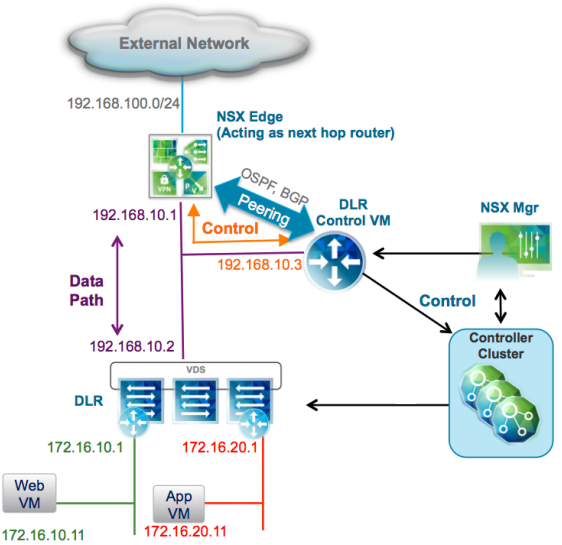
\includegraphics[width=0.4\textwidth]{imaxes/conceptosPrevios/LogicalRoutingComponents.png}
    %   \caption{Componentes de la red virtual que intervienen en el enrutamiento del tráfico.}
    %   \label{fig:logicalRoutingCompo}
    % \end{figure}
    % \FloatBarrier
    
    % \begin{figure}[h!]
    %   \centering
    %   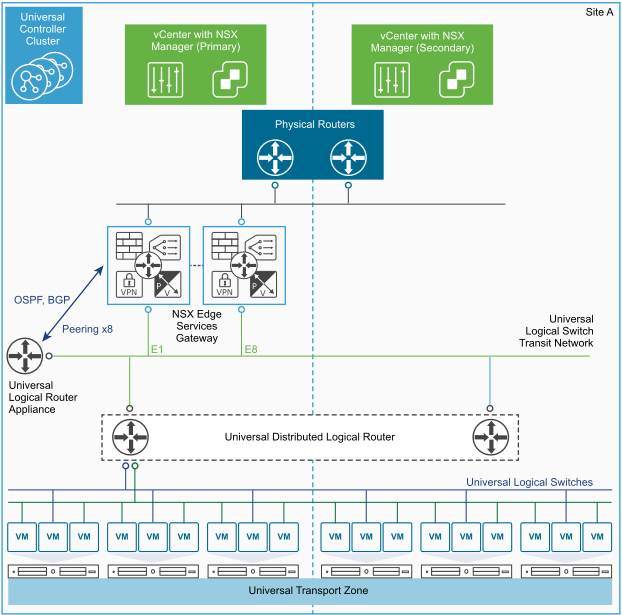
\includegraphics[width=0.5\textwidth]{imaxes/conceptosPrevios/redlogCF.png}
    %   \caption{Red lógica formada en un SDDC con dos clusters.}
    %   \label{fig:redLogicaOne}
    % \end{figure}
    % \FloatBarrier
     
    %  En el SDDC deben existir, al menos, dos intancias de ESG aunque se pueden desplegar hasta 8 instancias. En el modelo consolidado se debe tener un único UDLR para que las rutas entre hosts ESXi sean más cortas, debe existir un Logical Switch que forme la \textit{transit zone}. En el modelo estándar debe existir un UDLR extendido por todos los \textit{Management Cluster} (si hay varias \textit{Regions}), un UDLR extendido por el \textit{Shared Edge and Compute Cluster} y el resto de \textit{Compute Clusters} en cada \textit{Region}, y un DLR extendido por todos los clusters de una misma región.En el modelo estándar existen dos tipos de \textit{transit zones}, una entre el UDLR que atraviesa todas las \textit{Regions} y cada instancia de ESG, y otra que conecta el DLR propio de cada \textit{Region} y sus instancias de ESG. 
    % \\
    % Algunos componentes de VMware Cloud Foundation se deben desplegar en una VXLAN dedicada para proporcionar recuperación ante fallos en caso de que parte del SDDC deje de funcionar. Entre otros componentes (solo vamos a tratar aquellos que son obligatorios), VMware vRealize Log Insight se debe desplegar en una red de este tipo, llamada \textit{Application Virtual Network} (AVN). En entornos con varias \textit{Regions} se crea una \textit{transport zone} que se extiende por todo el SDDC y una \textit{transport zone} adicional en cada \textit{Region}, la primera proporciona recuperación ante fallos a través de todo el SDDC a los componentes que lo requieran, y la segunda solo a través de una \textit{Region}, sin necesidad de reconfigurar direcciones IP o DNS. VMware vRealize Log Insight se debe desplegar en una VXLAN por cada \textit{Region}.
    % \\
    % El acceso a una AVN se realiza a través de las instancias de ESG desplegadas en el entorno, estas se conectan a un UDLR que gestiona el tráfico de la s máquinas virtuales que tiene conectadas. El enrutamiento debe ser dinámico con BGP y las instancias de ESG proporcionan protegen y balacean la carga de trabajo con los servicios de VMware NSX Firewall y Load Balancing [Fig. \ref{fig:avnConsolidated}].\\
    % **VERIFICAR LO DEL LOAD BALANCING en el despliegue. ¿solo para las que son cross-region o tambien en las de una sola region**\\
    % \begin{figure}[h!]
    %   \centering
    %   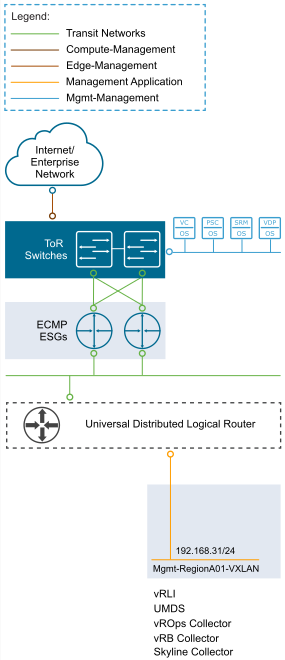
\includegraphics[width=0.25\textwidth]{imaxes/conceptosPrevios/AVNConsolidated.png}
    %   \caption{AVN en el modelo consolidado}
    %   \label{fig:avnConsolidated}
    % \end{figure}
    % \FloatBarrier
    
    % Este utiliza los componentes vCenter Server, NSX Manager, NSX Controllers y NSX Logical Switch para establecer comunicaciones y aislar los distintos tipos de tráfico [Fig. \ref{fig:planosNSX}]. Estos componentes \underline{actúan en diferentes planos} de la red:
    
    
    
    % \begin{itemize}
    %     \item \textbf{Plano de Datos}: esta capa gestiona la transmisión del tráfico entre los componentes del SDDC. En este plano actúan NSX Logical Switches segregando los tipos de datos, y el enrutamiento y firewall distribuído de NSX. Se transmite a través de una red física dedicada al transporte.
    %     \item \textbf{Plano de Control}: aquí se gestionan los mensajes de control que se usan para la configuración de los dispositivos de NSX como switches, routers y firewalls en cada host ESXi. Se distribuye en redes físicas de forma segura usando VLANs para aislarlo del plano de datos.
    %     \item \textbf{Plano de gestión}: aquí se gestiona el tráfico dedicado a la administración de los recursos como puede ser la creación y eliminación de máquinas virtuales. Está controlado por vCenter Server y NSX Manager.
    % \end{itemize}
    % \begin{figure}[h!]
    %   \centering
    %   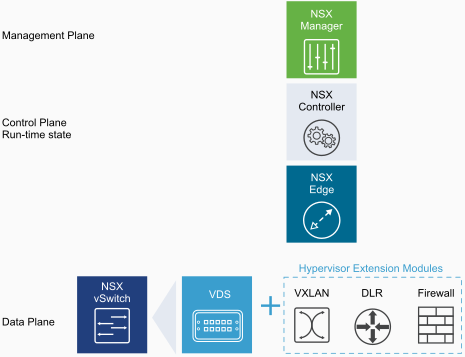
\includegraphics[width=0.65\textwidth]{imaxes/conceptosPrevios/planosNSX.png}
    %   \caption{Como se estructuran las componentes de VMware NSX for vSphere}
    %   \label{fig:planosNSX}
    % \end{figure}
    % \FloatBarrier
    
    %\fi
    
    % \iffalse
    % \subsubsection{Almacenamiento Virtual}
    % VMware vSAN forma único \textit{datastore} con todos los dispositivos de almacenamiento que se encuentran en la infraestructura permitiendo establecer políticas y gestionar esos recursos de forma más simple. Para que funcione correctamente es necesario \underline{configurar una red para VMware vSAN} teniendo en cuenta los siguientes aspectos:
    % \begin{itemize}
    %     \item El uso de vSpehere Distributed Switches genera mejor rendimiento.
    %     \item Se recomienda el uso de paquetes tipo \textit{jumbo frames}.
    %     \item Asignar una VLAN al tráfico de cada cluster de VMware vSAN.
    %     \item Si se implementa en un SDDC con dos localizaciones, es necesario establecer un host \textit{witness}.
    % \end{itemize}
    % Al establecer el tamaño y capacidad de este cluster hay que tener en cuenta que cuantos más hosts ESXi se incluyan, mayor tolerancia a fallos se tendrá y mejor se podrán repartir los grupos de discos entre todos los hosts. Debe haber un balance entre el hardware y la capacidad requerida.
    
    
    % \fi